\documentclass[12pt]{article}
\usepackage{graphicx}
\usepackage{enumitem}
\usepackage{amsmath}
\usepackage{gvv-book}
\usepackage{gvv}

\title{\textbf{4.13.10}}
\author{\textbf{Aditya Mishra-EE25BTECH11005}}
\date{October 3, 2025}

\begin{document}

\maketitle

\section*{Question}
\[
\vec{A} = \myvec{-1\\-7},\quad
\vec{B} = \myvec{5\\1},\quad
\vec{C} = \myvec{1\\10}
\]
Equation of the internal bisector of $\angle ABC$.

\section*{Solution}

\[
\text{Given lines } \vec{n}_1^{\top} \vec{x} = c_1, \quad \vec{n}_2^{\top} \vec{x} = c_2,
\]

\[
\text{Angle bisectors satisfy }
\frac{|\vec{n}_1^{\top} \vec{x} - c_1|}{\|\vec{n}_1\|}
= \frac{|\vec{n}_2^{\top} \vec{x} - c_2|}{\|\vec{n}_2\|}.
\]

\[
\Rightarrow \quad
\frac{\vec{n}_1^{\top} \vec{x} - c_1}{\|\vec{n}_1\|}
= \pm \frac{\vec{n}_2^{\top} \vec{x} - c_2}{\|\vec{n}_2\|}.
\]

\[
\text{Internal bisector: sign chosen so that for }
\vec{u} =
\frac{\vec{A}-\vec{B}}{\|\vec{A}-\vec{B}\|}
+
\frac{\vec{C}-\vec{B}}{\|\vec{C}-\vec{B}\|},
\quad
\text{we have }
\operatorname{sgn}(\vec{n}_1^{\top} \vec{u}) = -\operatorname{sgn}(\vec{n}_2^{\top} \vec{u})
\]

Normals:
\begin{align}
\vec{n}_1 &= \myvec{-8\\6} \\
\vec{n}_2 &= \myvec{9\\4}
\end{align}
Norms:
\begin{align}
\|\vec{n}_1\| &= \sqrt{(-8)^2 + 6^2} = 10 \\
\|\vec{n}_2\| &= \sqrt{9^2 + 4^2} = \sqrt{97}
\end{align}
Equation of angle bisector:
\[
\frac{\vec{n}_1^{\top} (\vec{x} - \vec{B})}{10}
=
-\frac{\vec{n}_2^{\top} (\vec{x} - \vec{B})}{\sqrt{97}}
\]
Thus,
\[
\sqrt{97}\,\vec{n}_1^{\top} (\vec{x} - \vec{B}) + 10\,\vec{n}_2^{\top} (\vec{x} - \vec{B}) = 0
\]

With
$\vec{B} = \myvec{5\\1}$, equation of Angle Bisector is:

\begin{align*}
\boxed{ \myvec{90-8\sqrt{97} \\ 40+6\sqrt{97}}^T \vec{x} + (34\sqrt{97}-490) = 0 }
\end{align*}

\text{Or,}
\begin{align*}
\boxed{\vec{x} = \myvec{5 \\ 1} + \lambda\myvec{40+6\sqrt{97} \\ -(90-8\sqrt{97})},\quad \lambda \in \mathbb{R}}
\end{align*}

\textbf{Plot}
\begin{figure}[H]
    \centering
    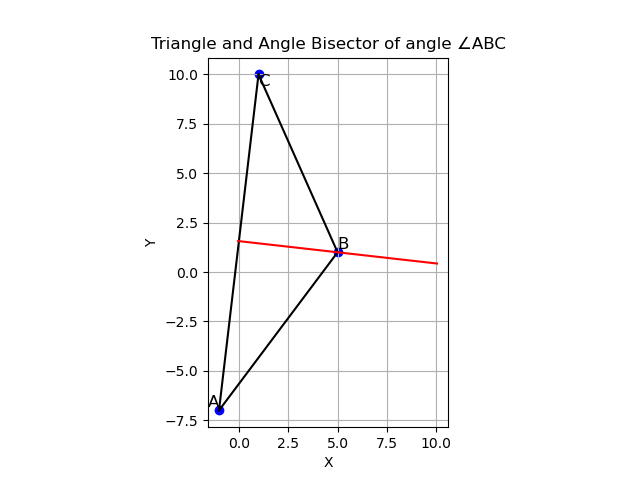
\includegraphics[width=0.8\columnwidth]{Figs/Figure_1.png}
\end{figure}

\end{document}

